%! Author = kyoto
%! Date = 08.03.2022


\section{Задание}
По выданному преподавателем варианту восстановить текст заданного варианта программы и подпрограммы
(программного комплекса), определить предназначение и составить его описание, определить область представления и область
допустимых значений исходных данных и результата, выполнить трассировку программного комплекса.


\begin{figure}[H]
    \centering
    
\includegraphics[scale=0.6]{img/variant}
\end{figure}


\section{Программа}

\subsection{Основная:}
\begin{center}
    \begin{tabular}{|c|c|c|l|}
        \hline
        \textbf{Cell Address} & \textbf{Cell Content} & \textbf{Mnemonics} & \textbf{Comments}                                    \\
        \hline
        1D9                   & + 0200                & CLA                & Очистка аккумулятора.                                \\
        1DA                   & EE1A                  & ST (IP+26)         & Сохранение аккумулятора в ячейку 1F5 (R).            \\
        1DB                   & AE18                  & LD (IP+24)         & Загрузка в аккумулятор данных из ячейки 1F4 (X).     \\
        1DC                   & 0700                  & INC                & Инкрементация значения в аккумуляторе.               \\
        1DD                   & 0C00                  & PUSH               & Загрузка содержимого AC в подпрограмму.              \\
        1DE                   & D71D                  & CALL 71D           & Вызов подпрограммы с началом в ячейке 71D.           \\
        1DF                   & 0800                  & POP                & Выгрузка результата подпрограммы в AC.               \\
        1E0                   & 6E14                  & SUB (IP+20)        & Вычитание из аккумулятора значение ячейки 1F5 (R).   \\
        1E1                   & EE13                  & ST (IP+19)         & Сохранение результата в ячейку 1F5 (R).              \\
        1E2                   & AE0F                  & LD (IP+15)         & Загрузка в аккумулятор данных из ячейки 1F2 (Z).     \\
        1E3                   & 0740                  & DEC                & Декрементация значения в аккумуляторе.               \\
        1E4                   & 0C00                  & PUSH               & Загрузка содержимого AC в подпрограмму.              \\
        1E5                   & D71D                  & CALL 71D           & Вызов подпрограммы в ячейке 71D.                     \\
        1E6                   & 0800                  & POP                & Выгрузка результата подпрограммы в AC.               \\
        1E7                   & 4E0D                  & ADD (IP+13)        & Сложение значения из ячейки 1F5 (R) с аккумулятором. \\
        1E8                   & EE0C                  & ST (IP+12)         & Сохранение результата в ячейку 1F5 (R).              \\
        1E9                   & AE09                  & LD (IP+9)          & Загрузка в аккумулятор значение из ячейки 1F3 (Y).   \\
        1EA                   & 0740                  & DEC                & Декрементация значения в аккумуляторе.               \\
        1EB                   & 0C00                  & PUSH               & Загрузка содержимого AC в подпрограмму.              \\
        1EC                   & D71D                  & CALL 71D           & Вызов подпрограммы в ячейке 71D.                     \\
        1ED                   & 0800                  & POP                & Выгрузка результата подпрограммы в AC.               \\
        1EE                   & 0740                  & DEC                & Декрементация значения в аккумуляторе.               \\
        1EF                   & 4E05                  & ADD (IP+5)         & Сложение с аккумулятором значения из ячейки 1F5 (R). \\
        1F0                   & EE04                  & ST (IP+4)          & Сохранение результата в ячейку 1F5 (R).              \\
        1F1                   & 0100                  & HLT                & Остановка.                                           \\
        \hline
        1F2                   & 0008                  & Z                  & Переменная Z. Значение 8.                            \\
        1F3                   & FFF1                  & Y                  & Переменная Y. Значение -15.                          \\
        1F4                   & FFEC                  & X                  & Переменная X. Значение -20.                          \\
        1F5                   & FDE8                  & R                  & Ячейка для хранения результата (R).                  \\
        \hline
    \end{tabular}
\end{center}


\newpage

\subsection{Подпрограмма:}
\begin{center}
    \begin{tabular}{|c|c|c|l|}
        \hline
        \textbf{Cell Address} & \textbf{Cell Content} & \textbf{Mnemonics} & \textbf{Comments}                                            \\
        \hline
        71D                   & AC01                  & LD (SP+1)          & Загрузка в аккумулятор последнего сохранённого в стек числа. \\
        71E                   & F001                  & BEQ (IP+1)         & IF Z==1 THEN 720 -> IP (skip next).                          \\
        71F                   & F304                  & BPL (IP+4)         & IF N==0 THEN 724 -> IP.                                      \\
        720                   & 6E0A                  & SUB (IP+10)        & AC-MEM(72B).                                                 \\
        721                   & F201                  & BMI (IP+1)         & IF N==1 THEN 723 -> IP (skip next).                          \\
        722                   & CE05                  & JUMP (IP+5)        & 728 -> IP.                                                   \\
        723                   & 4E07                  & ADD (IP+7)         & Сложение с аккумулятором значения из ячейки 72B (V).         \\
        724                   & 0500                  & ASL                & Арифметический сдвиг влево                                   \\
        725                   & 0500                  & ASL                & (AC_{15} -> C; AC_{i} = AC_{i-1}; 0 -> AC_{0}).              \\
        726                   & 6E05                  & SUB (IP+5)         & Вычитание из аккумулятора значение ячейки 72C (B).           \\
        727                   & CE01                  & JUMP (IP+1)        & 729 -> IP (skip next).                                       \\
        728                   & AE02                  & LD (IP+2)          & Загрузка в аккумулятор значения ячейки 72B (V).              \\
        729                   & EC01                  & ST (SP+1)          & Сохранение результата в стек (SP)+.                          \\
        72A                   & 0A00                  & RET                & Возвращение из подпрограммы.                                 \\
        \hline
        72B                   & FF06                  & V                  & Локальная переменная подпрограммы (-250).                    \\
        72C                   & 0027                  & B                  & Локальная переменная подпрограммы (39).                      \\
        \hline
    \end{tabular}
\end{center}


\section{Функция, реализуемая программой}

\subsection{Основная программа:}
\begin{center}
    \textit{R (X, Y, Z) = F(X+1) + F(Z-1) + F(Y-1) - 1 .}
\end{center}

\subsection{Подпрограмма:}
\begin{center}
    \begin{equation*}
        \textit{
            F(t)=
            \begin{cases}
                4t - 39 &\text{, if t < -250 ;}\\
                -250 &\text{, if -250 $\leqslant$ t $\leqslant$ 0 ;}\\
                4t - 39 &\text{, if t > 0 .}\\
            \end{cases}
        }
    \end{equation*}
\end{center}

\subsection{График функции подпрограммы:}
\begin{figure}[H]
    \centering
    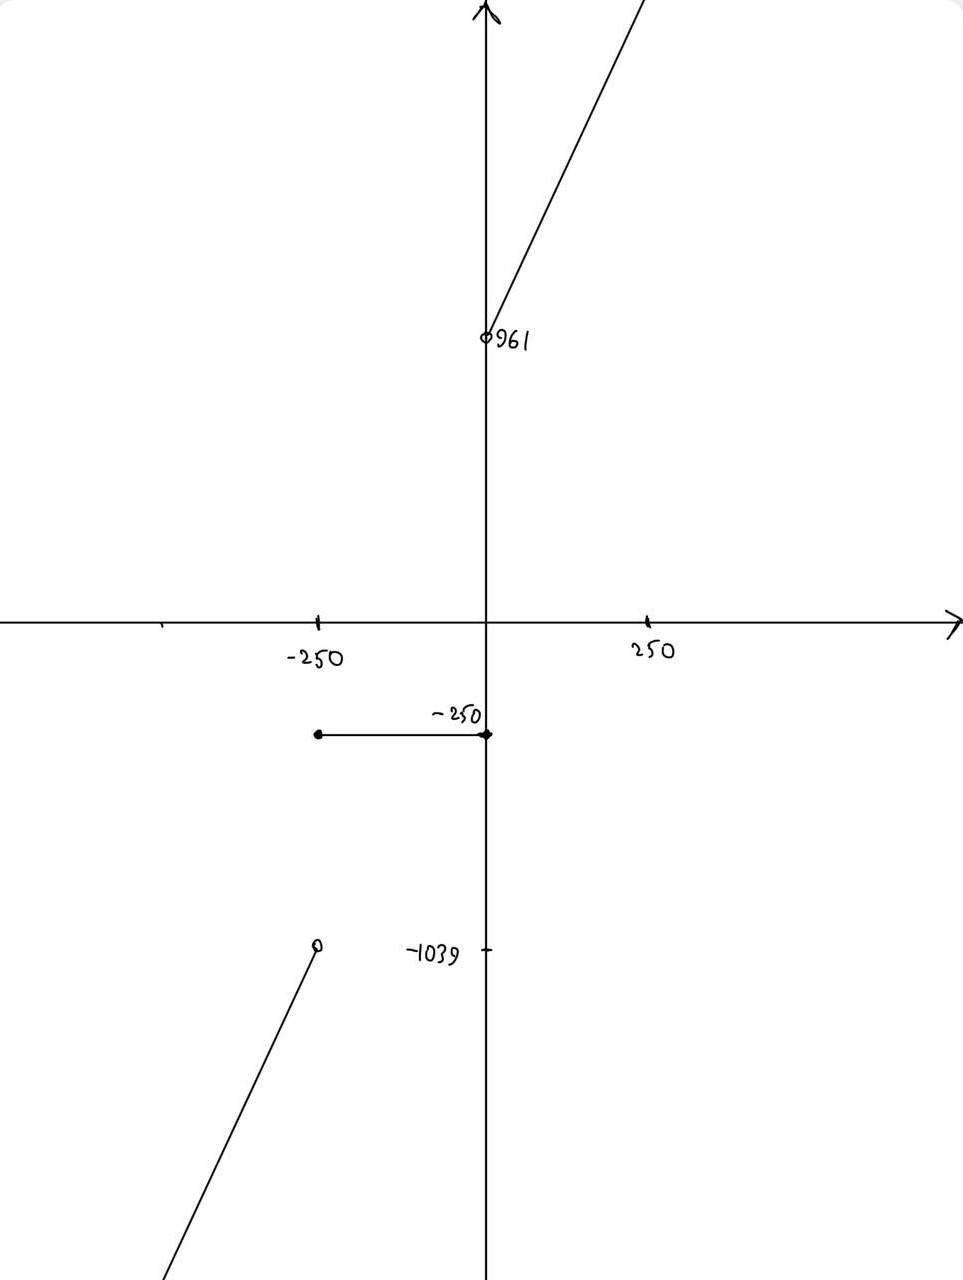
\includegraphics[scale=0.3]{img/graphic}
\end{figure}

\newpage


\section{Область представления данных и область допустимых значений}

\subsection{Область представления:}
В ячейках X, Y, Z, V, B, R находятся знаковые 16теричные целые числа.

\subsection{ОДЗ}

\subsubsection{Подпрограммы:}
\begin{equation*}
    \begin{center}
        F(x) $\in$ [$\frac{-2^{15}+1}{3}$;$\frac{2^{15}}{3}$]
    \end{center}
\end{equation*}

\subsubsection{X:}
\begin{equation*}
    \begin{center}
        $\frac{-2^{15}+118}{12} - 1 \leqslant X \leqslant \frac{2^{15}+117}{12} - 1$\\
        or\\
        $-2721 \leqslant X \leqslant 2739 $
    \end{center}
\end{equation*}

\subsubsection{Y:}
\begin{equation*}
    \begin{center}
        $\frac{-2^{15}+118}{12} + 1 \leqslant Y \leqslant \frac{2^{15}+117}{12} + 1$\\
        or\\
        $-2719 \leqslant Y \leqslant 2741 $
    \end{center}
\end{equation*}

\subsubsection{Z:}
\begin{equation*}
    \begin{center}
        $\frac{-2^{15}+118}{12} + 1 \leqslant Z \leqslant \frac{2^{15}+117}{12} + 1$\\
        or\\
        $-2719 \leqslant Z \leqslant 2741 $
    \end{center}
\end{equation*}

\subsubsection{Результата:}
\begin{equation*}
    \begin{center}
        $-2^{15} \leqslant R \leqslant 2^{15}-1$
    \end{center}
\end{equation*}


\section{Расположение программы в памяти БЭВМ:}
\noindent\textit{Основной программы - \textbf{1D9-1F1} . \\
Первый аргумент программы – \textbf{1F2} .  \\
Второй аргумент программы – \textbf{1F3} .  \\
Третий аргумент программы – \textbf{1F4} .  \\
Результат программы – \textbf{1F5} .    \\
Подпрограммы – \textbf{71D-72A} .   \\
Вспомогательная переменная подпрограммы – \textbf{72B} .    \\
Вспомогательная переменная подпрограммы – \textbf{72C} .    \\}

\newpage

\section {Трассировка}

\begin{figure}[H]
    \centering
    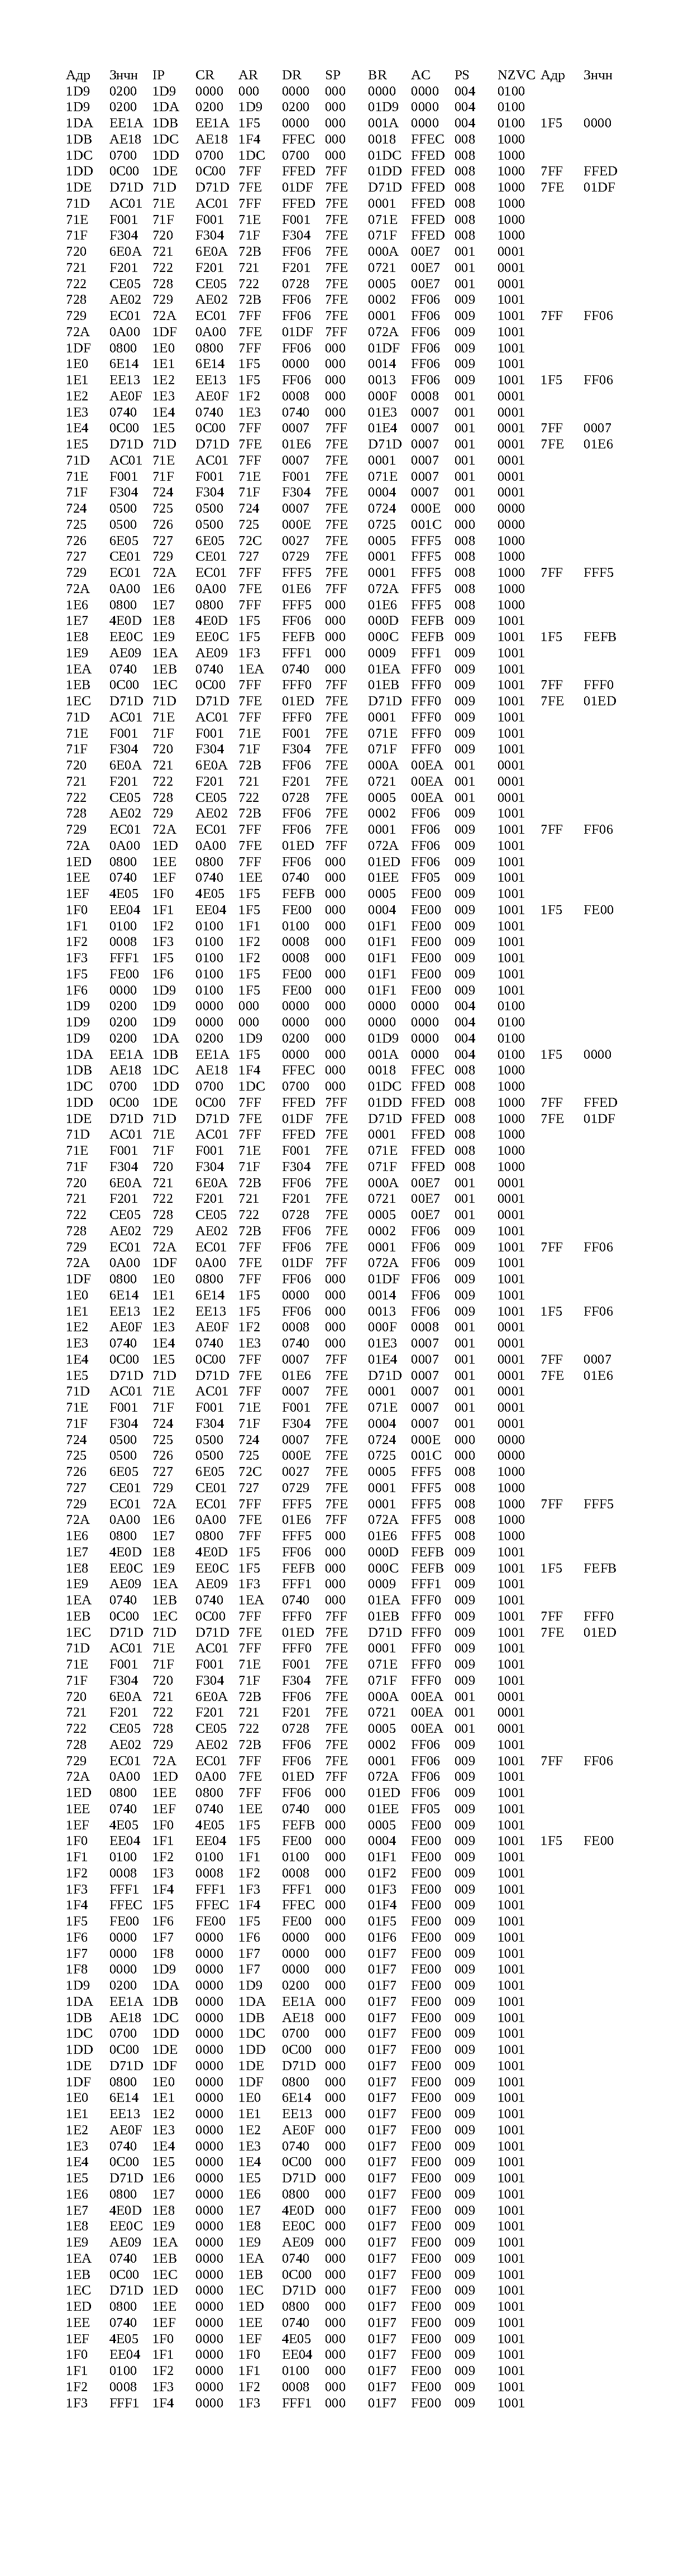
\includegraphics[scale=0.32]{img/trss}
\end{figure}

\subsection{Проверка программы:}
\noindent
F(-20+1) = -250 ; \\
F(8-1) = 7*4 - 39 = -11 ; \\
F(-15-1) = -250 ; \\
Result = (-250) + (-11) + (-250) - 1 = -512 = FE00 . \\


\section{Доп. задание}
\textit{
Написать программу, реализующую пробег по двум массивам, сравнивая объекты в них: если i-ый номер во втором массиве
равен нулю, то i-тый номер в первом массиве необходимо записать.}

\subsection{Программа}
\begin{center}
    \begin{tabular}{|c|c|c|l|}
        \hline
        \textbf{Cell Address} & \textbf{Cell Content} & \textbf{Mnemonics} & \textbf{Comments}                                 \\
        \hline
        001                   & 0016                  & Addr $M_{1}$       & Адрес начала массива №1                           \\
        002                   & 001B                  & Addr $M_{2}$      & Адрес начала массива №2                           \\
        003                   & FFFF                  & $M_{1,i}$ caller   & Ячейка, в которую сохраняется адрес для обращения \\
        &                       &                    & к элементу массива №1                             \\
        004                   & FFFF                  & $M_{2}$ caller     & Ячейка, в которую сохраняется адрес для обращения \\
        &                       &                    & к элементу массива №2                             \\
        005                   & FFFF                  & iterator           & Итератор цикла                                    \\
        006                   & +0200                 & CLA                & Очистка аккумулятора                              \\
        007                   & AF05                  & LD #5              & Прямая загрузка числа 5 в AC                      \\
        008                   & E005                  & ST 5               & Сохранение 5 в ячейку итератора                   \\
        009                   & 4002                  & ADD 2              & AC + Адрес начала $M_{2}$                           \\
        00A                   & E004                  & ST 4               & Сохранить AC в $M_{2}$ caller                       \\
        00B                   & ABF8                  & LD -(IP-8)         & Загрузка в аккумулятор значения, на которую       \\
        &                       &                    & указывает $M_2$ caller с предекрементом           \\
        00C                   & F106                  & BNE 6              & IF Z == 0 THEN IP+6                               \\
        00D                   & A001                  & LD 1               & Загрузка в AC адреса начала массива №1            \\
        00E                   & 0740                  & DEC                & Декрементация значения в AC                       \\
        00F                   & 4005                  & ADD 5              & AC + iterator                                     \\
        010                   & E003                  & ST 3               & Сохранить AC в $M_{1,i}$ caller                     \\
        011                   & A8F1                  & LD (IP-15)         & Загрузка в аккумулятор ячейки, на которую         \\
        &                       &                    & указывает $M_{1,i}$ caller                        \\
        012                   & 0C00                  & PUSH               & Запись в стек значения из аккумулятора            \\
        013                   & 8005                  & LOOP 5             & LOOP итератора                                    \\
        014                   & C00B                  & JUMP 00B           & Возврат на ячейку 00B для следующего цикла        \\
        015                   & 0100                  & HLT                & Остановка программы                               \\
        \hline
        016                   & 0001                  & $M_{1,1}$          &                                                   \\
        017                   & 0002                  & $M_{1,2}$          &                                                   \\
        018                   & 0003                  & $M_{1,3}$          &                                                   \\
        019                   & 0004                  & $M_{1,4}$          &                                                   \\
        01A                   & 0005                  & $M_{1,5}$          &                                                   \\
        \hline
        01B                   & 00FF                  & $M_{2,1}$          &                                                   \\
        01C                   & 0000                  & $M_{2,2}$          &                                                   \\
        01D                   & 5555                  & $M_{2,3}$          &                                                   \\
        01E                   & 0000                  & $M_{2,4}$          &                                                   \\
        01F                   & 1234                  & $M_{2,5}$          &                                                   \\
        \hline
    \end{tabular}
\end{center}

\subsection{Описание программы:}
\textit{
Пробегает по массиву №2, если i-ый элемент равен нулю, то она вычисляет адрес i-го элемента в массиве №1, загружает
его в аккумулятор и записывает в стек. По завершении программы в стеке лежит список элементов массива №1, порядковый
номер которых соответствует нулю в массиве №2}